\documentclass{article}
\usepackage{fancyhdr}
\usepackage{amsmath}
\usepackage{tikz}
\usepackage{xcolor}
\usepackage{pgfplots}
\usepackage{pst-func}
\usepackage{mathrsfs}
\usepackage{graphicx}
\usepackage{subfigure}
\usepackage{float}
\pagestyle{fancy}
\setlength{\headheight}{35pt}
\lhead{Machine Learning\\Sommersemester2020\\Exercise 5}
\chead{}
% bfseries
\rhead{Ciheng Zhang(3472321)\\Gang Yu(3488292)\\Huibanjun Tian(3471607)}
\cfoot{\thepage}
\renewcommand{\headrulewidth}{0.4pt}

\begin{document}
\begin{titlepage}
    \title{\Huge \textbf{Machine Learning\\Sommersemester2020\\Exercise 5} }
    \author{\LARGE \textsl{Ciheng Zhang (3472321) zch3183505@gmail.com}\\\LARGE \textsl{Gang Yu(3488292) HansVonCq@gmail.com}\\\LARGE \textsl{Huipanjun Tian (3471607)  Thpjpyl5111217@gmail.com} \\[200pt]}
    \date{\today}
    \maketitle
    \thispagestyle{empty}
\end{titlepage}
\newpage
\section{Inductive Construction}
according to the table, At first we calculate the Entropy of the dataset.
\[P(-)=\frac{125}{240} P(+)=\frac{115}{240}\]
\[Ent(D)=-(P(-)log_2(P(-))+P(+)log_2(p(+)))=0.9987\]
Then we try try to divide the dataset by different features and calculate the Gain of each features, and choose one feature to divide the dataset.
\\BY F1:\\
\begin{center}
    \begin{tabular}{cc}
    F1=0\\
    \hline
    -&+\\
    \hline
    70&50\\
    \hline
\end{tabular}
\begin{tabular}{cc}
    F1=1\\
    \hline
    -&+\\
    \hline
    55&65\\
    \hline
\end{tabular}
\end{center}
\[Ent(F1=0)=0.9798\]
\[Ent(F1=1)=0.9950\]
\[Gain(F1)=Ent(D)-\frac{D(F1=0)}{D}Ent(F1=0)-\frac{D(F1=1)}{D}Ent(F1=1)=0.0113\]
\\BY F2:\\
\begin{center}
    \begin{tabular}{cc}
    F2=0\\
    \hline
    -&+\\
    \hline
    50&70\\
    \hline
\end{tabular}
\begin{tabular}{cc}
    F2=1\\
    \hline
    -&+\\
    \hline
    75&45\\
    \hline
\end{tabular}
\end{center}
\[Ent(F2=0)=0.9798\]
\[Ent(F2=1)=0.9944\]
\[Gain(F2)=0.0116\]
\\BY F3:\\
\begin{center}
    \begin{tabular}{cc}
    F3=0\\
    \hline
    -&+\\
    \hline
    65&15\\
    \hline
\end{tabular}
\begin{tabular}{cc}
    F3=1\\
    \hline
    -&+\\
    \hline
    50&30\\
    \hline
\end{tabular}
\begin{tabular}{cc}
    F3=2\\
    \hline
    -&+\\
    \hline
    10&70\\
    \hline
\end{tabular}
\end{center}
\[Ent(F3=0)=0.6962\]
\[Ent(F3=1)=0.9544\]
\[GEnt(F3=2)=0.5436\]
\[Gain(F3)=0.2673\]
\newpage
BY F4:\\
\begin{center}
    \begin{tabular}{cc}
    F4=0\\
    \hline
    -&+\\
    \hline
    70&50\\
    \hline
\end{tabular}
\begin{tabular}{cc}
    F2=1\\
    \hline
    -&+\\
    \hline
    65&65\\
    \hline
\end{tabular}
\end{center}
\[Ent(F2=0)=0.9798\]
\[Ent(F2=1)=1\]
\[Gain(F2)=0.008\]
because of $Gain(F3)>Gain(F2)>Gain(F1)>Gain(F4)$,we choose F3 as the feature:\\
\begin{center}
    \begin{tikzpicture}[sibling distance=10em,
    every node/.style = {shape=rectangle, rounded corners,
      draw, align=center,
      top color=white, bottom color=blue!20}]]
    \node {F3}
      child { node[label={above:F3=0}]{  }}
      child { node[label={above:F3=1}]{  }}  
      child { node[label={above:F3=2}]{  }};
  \end{tikzpicture}
\end{center}
Then we rebulid the table for each Note:\\

\begin{tabular}{|ccc|cc|}
    F3&=0\\
    \hline
    F1&F2&F4&-&+\\
    \hline
    0&0&0&10&0\\
    0&0&1&5&5\\
    0&1&0&10&0\\
    0&1&1&10&0\\
    1&0&0&0&10\\
    1&0&1&10&0\\
    1&1&0&10&0\\
    1&1&1&10&0\\
    \hline
\end{tabular}
\begin{tabular}{|ccc|cc|}
    F3&=1\\
    \hline
    F1&F2&F4&-&+\\
    \hline
    0&0&0&10&0\\
    0&0&1&10&0\\
    0&1&0&5&5\\
    0&1&1&0&10\\
    1&0&0&5&5\\
    1&0&1&0&10\\
    1&1&0&10&0\\
    1&1&1&10&0\\
    \hline
\end{tabular}
\begin{tabular}{|ccc|cc|}
    F3&=2\\
    \hline
    F1&F2&F4&-&+\\
    \hline
    0&0&0&0&10\\
    0&0&1&0&10\\
    0&1&0&10&0\\
    0&1&1&0&10\\
    1&0&0&0&10\\
    1&0&1&0&10\\
    1&1&0&0&10\\
    1&1&1&0&10\\
    \hline
\end{tabular}\\
% 计算节点流程复制就行
Then we calculate for the first Node(F3=0):\\
\[Ent(F3=0)=0.6962\]
\\BY F1:\\
\begin{center}
    \begin{tabular}{cc}
    F1=0\\
    \hline
    -&+\\
    \hline
    35&5\\
    \hline
\end{tabular}
\begin{tabular}{cc}
    F1=1\\
    \hline
    -&+\\
    \hline
    30&10\\
    \hline
\end{tabular}
\end{center}
\[Ent(F1=0)=0.5435\]
\[Ent(F1=1)=0.8112\]
\[Gain(F2)=0.01885\]
\\BY F2:\\
\begin{center}
    \begin{tabular}{cc}
    F2=0\\
    \hline
    -&+\\
    \hline
    25&15\\
    \hline
\end{tabular}
\begin{tabular}{cc}
    F2=1\\
    \hline
    -&+\\
    \hline
    40&0\\
    \hline
\end{tabular}
\end{center}
\[Ent(F2=0)=0.9544\]
\[Ent(F1=1)=0\]
\[Gain(F2)=0.219\]
\\BY F4:\\
\begin{center}
    \begin{tabular}{cc}
    F4=0\\
    \hline
    -&+\\
    \hline
    30&10\\
    \hline
\end{tabular}
\begin{tabular}{cc}
    F4=1\\
    \hline
    -&+\\
    \hline
    35&5\\
    \hline
\end{tabular}
\end{center}
\[Ent(F4=0)=0.8112\]
\[Ent(F4=1)=0.5435\]
\[Gain(F4)=0.01885\]
because of $Gain(F2)>Gain(F1)=Gain(F4)$,we choose F2 as the feature:
\begin{center}
    \begin{tikzpicture}[sibling distance=10em,
    every node/.style = {shape=rectangle, rounded corners,
      draw, align=center,
      top color=white, bottom color=blue!20}]]
    \node {F3}
      child { node[label={above:F3=0}]{F2}
                child{node[label={above:F2=0}]{-}}
                child{node[label={above:F2=1}]{-}}}
      child { node[label={above:F3=1}]{  }}  
      child { node[label={above:F3=2}]{  }};
  \end{tikzpicture}
\end{center}
% 计算节点流程复制就行
Then we calculate for the second Node(F3=1):\\
\[Ent(F3=1)=0.9544\]
\\BY F1:\\
\begin{center}
    \begin{tabular}{cc}
    F1=0\\
    \hline
    -&+\\
    \hline
    25&15\\
    \hline
\end{tabular}
\begin{tabular}{cc}
    F1=1\\
    \hline
    -&+\\
    \hline
    25&15\\
    \hline
\end{tabular}
\end{center}
\[Ent(F1=0)=0.9544\]
\[Ent(F1=1)=0.9544\]
\[Gain(F1)=0\]
\\BY F2:\\
\begin{center}
    \begin{tabular}{cc}
    F2=0\\
    \hline
    -&+\\
    \hline
    25&15\\
    \hline
\end{tabular}
\begin{tabular}{cc}
    F2=1\\
    \hline
    -&+\\
    \hline
    25&15\\
    \hline
\end{tabular}
\end{center}
\[Ent(F2=0)=0.9544\]
\[Ent(F2=1)=0.9544\]
\[Gain(F2)=0\]
\\BY F4:\\
\begin{center}
    \begin{tabular}{cc}
    F4=0\\
    \hline
    -&+\\
    \hline
    30&10\\
    \hline
\end{tabular}
\begin{tabular}{cc}
    F4=1\\
    \hline
    -&+\\
    \hline
    20&20\\
    \hline
\end{tabular}
\end{center}
\[Ent(F4=0)=0.8112\]
\[Ent(F4=1)=1\]
\[Gain(F4)=0.0488\]
because of $Gain(F4)>Gain(F1)=Gain(F2)$,we choose F4 as the feature:
\begin{center}
    \begin{tikzpicture}[sibling distance=10em,
    every node/.style = {shape=rectangle, rounded corners,
      draw, align=center,
      top color=white, bottom color=blue!20}]]
    \node {F3}
      child { node[label={above:F3=0}]{F2}
                child{node[label={above:F2=0}]{-}}
                child{node[label={above:F2=1},xshift=-2em]{-}}}
      child { node[label={above:F3=1}]{F4}
                child{node[label={above:F4=0},,xshift=2em]{-}}
                child{node[label={above:F4=1}]{+}}}  
      child { node[label={above:F3=2}]{  }};
  \end{tikzpicture}
\end{center}
% 计算节点流程复制就行
Then we calculate for the second Node(F3=2):\\
\[Ent(F3=2)=0.5436\]
\\BY F1:\\
\begin{center}
    \begin{tabular}{cc}
    F1=0\\
    \hline
    -&+\\
    \hline
    10&30\\
    \hline
\end{tabular}
\begin{tabular}{cc}
    F1=1\\
    \hline
    -&+\\
    \hline
    0&40\\
    \hline
\end{tabular}
\end{center}
\[Ent(F1=0)=0.8113\]
\[Ent(F1=1)=0\]
\[Gain(F1)=0.1379\]
\\BY F2:\\
\begin{center}
    \begin{tabular}{cc}
    F2=0\\
    \hline
    -&+\\
    \hline
    0&40\\
    \hline
\end{tabular}
\begin{tabular}{cc}
    F2=1\\
    \hline
    -&+\\
    \hline
    10&30\\
    \hline
\end{tabular}
\end{center}
\[Ent(F2=0)=0.8113\]
\[Ent(F2=1)=0\]
\[Gain(F2)=0.1379\]
\\BY F4:\\
\begin{center}
    \begin{tabular}{cc}
    F4=0\\
    \hline
    -&+\\
    \hline
    10&30\\
    \hline
\end{tabular}
\begin{tabular}{cc}
    F4=1\\
    \hline
    -&+\\
    \hline
    0&40\\
    \hline
\end{tabular}
\end{center}
\[Ent(F4=0)=0.8113\]
\[Ent(F4=1)=0\]
\[Gain(F4)=0.1379\]
because of $Gain(F4)=Gain(F1)=Gain(F2)$,we choose F4 as the feature:
\begin{center}
    \begin{tikzpicture}[sibling distance=10em,
    every node/.style = {shape=rectangle, rounded corners,
      draw, align=center,
      top color=white, bottom color=blue!20}]]
    \node {F3}
      child { node[label={above:F3=0}]{F2}
                child{node[label={above:F2=0}]{-}}
                child{node[label={above:F2=1},xshift=-2em]{-}}}
      child { node[label={above:F3=1}]{F4}
                child{node[label={above:F4=0},xshift=2em]{-}}
                child{node[label={above:F4=1},xshift=-2em]{ +}}}  
      child { node[label={above:F3=2}]{F4}
                child{node[label={above:F4=0},xshift=2em]{+}}
                child{node[label={above:F4=1}]{+}}};
  \end{tikzpicture}
\end{center}
So we calculate the error rate for this tree:
\[ E=\frac{55}{240}=0.229\]
\newpage
\section{Minimal Error Pruning}
First we calculate the error rate of original tree:\\
\[E(origal)=\frac{1}{n(T)}\Sigma_{t\in T}e(t)=0.00615\]
Then first time Pruning:
\begin{figure}[H]
    \centering
    \includegraphics[width=0.8\textwidth]{pruningVier_1.png}
\end{figure}
Then we calculate the Error rate:\\
\[E(P1)=0.0371\]
\begin{figure}[H]
    \centering
    \includegraphics[width=0.8\textwidth]{pruningVier_2.png}
\end{figure}
Then we calculate the Error rate:\\
\[E(P2)=0.0061\]
\begin{figure}[H]
    \centering
    \includegraphics[width=0.8\textwidth]{pruningVier_3.png}
\end{figure}
Then we calculate the Error rate:\\
\[E(P3)=0.0106\]

\begin{figure}[H]
    \centering
    \includegraphics[width=0.8\textwidth]{purningVier_4.png}
\end{figure}
\[E(P4)=0.107\]
because of$E(P2)<E(P3)<E(P1)$ we Pruning the second viable node,and get the new tree:\\
\begin{figure}[H]
    \centering
    \includegraphics[width=0.8\textwidth]{pruningVier_2.png}
\end{figure}
Then we calculate for new viable node:\\
\begin{figure}[H]
    \centering
    \includegraphics[width=0.8\textwidth]{pruningDrei_1.png}
\end{figure}
\[E(P5)=0.0106\]
because of $E(P5)=E(P3)<others$  we prun the viable node of last time. and become a new tree:
\begin{figure}[H]
    \centering
    \includegraphics[width=0.8\textwidth]{pruningDrei_1.png}
\end{figure}
Then we repeat the uper method:
\begin{figure}[H]
    \centering
    \includegraphics[width=0.8\textwidth]{pruningZwei_1.png}
\end{figure}
\[E(P6)=0.0132\]
then we need to remove the node of last time. because $E(P6)<others$. 
And we get the final tree:
\begin{figure}[H]
    \centering
    \includegraphics[width=0.8\textwidth]{pruningZwei_1.png}
    \caption{Final Tree}
\end{figure}
\section{Regression with Decision Tress and kNN}
A regression tree is aim to one regression space. The classification tree's Node is features, and the viable node of classification tree is Tags of classification.
But all of the regression tree'node is a regression vlaue, and the viable node of the regression tree is the best regression value.
Then when we want to bulid a regression tree, we need to transver all the input values and calculate the distance.And we use the distance to bulid a loss function.
Then we Minimal the loss function and get the vlaue of next node. But for a classification tree we calculate and compare the Entropy Gain to decide the next Node.
\\
\\
A kNN use for a regression problem, at first we need to calculate a point and get the nearest k points. Then the output values is the mean value of those k nearest points.
Then we fit all of the output points and solve a regression problem.

\begin{thebibliography}{99}  
    \bibitem{ref1} https://blog.csdn.net/u012328159/article/details/70184415  
    \bibitem{ref2} https://www.jianshu.com/p/7c385f268bf9
    \bibitem{ref2} https://blog.csdn.net/on2way/article/details/88673075
\end{thebibliography}
\end{document}